\documentclass{beamer}
\usepackage[utf8]{inputenc}
\usepackage[slovak]{babel}
\usetheme{Szeged}
\usecolortheme{wolverine}

\makeatletter
\setbeamertemplate{footline}
{
  \leavevmode%
  \hbox{%
  \begin{beamercolorbox}[wd=.15\paperwidth,ht=2.25ex,dp=1ex,center]{author in head/foot}%
    Anton Kica
  \end{beamercolorbox}%
  \begin{beamercolorbox}[wd=.75\paperwidth,ht=2.25ex,dp=1ex,center]{title in head/foot}%
    \inserttitle
  \end{beamercolorbox}%
  \begin{beamercolorbox}[wd=.10\paperwidth,ht=2.25ex,dp=1ex,right]{date in head/foot}%
    \insertframenumber{} / \inserttotalframenumber\hspace*{2ex} 
  \end{beamercolorbox}}%
  \vskip0pt%
}
\makeatother%% only for this example, otherwise in .bib file

\usepackage{biblatex}
\addbibresource{literatura.bib}

\title{Systém na podporu vypracovania bezpečnostných projektov pre malé ISVS}
\author{
    {Anton Kica} \\
    {\and} \\
    {\textit{Školiteľ}} \\
    {doc. RNDr. Daniel Olejár, PhD., mim. prof.}
}

\begin{document}

\section{Úvod}
\frame{\titlepage}
\institute{FMFI Matfyz}
\date{2024}

%\begin{frame}
%  \begin{quote}
%    Internet sa chystá zabíjať ľudí a vláda reguluje veci, ktoré zabíjajú ľudí.
%  \end{quote}(preložené z angl.)
%  {\hfill \normalfont \scriptsize \textit{Bruce Schneier}}
%\end{frame}

\begin{frame}
  \frametitle{Informatizácia spoločnosti}

  \begin{itemize}
    \item veľké množstvo údajov
    \item digitálne informačné a komunikačné technológie
    \item potreba ochrany v tzv. kybernetickom priestore
    \item zákon o kybernetickej bezpečnosti (69/2018 Z. z.)
    \item zákon o informačných technológiách vo verejnej správe (95/2019 Z. z.)
  \end{itemize}

\end{frame}

\begin{frame}
  \frametitle{To najdôležitejšie z právnych predpisov}
  \begin{itemize}
    \item určenie manažéra kybernetickej a informačnej bezpečnosti
    \item zavedenie systému riadenia informačnej bezpečnosti
  \end{itemize}
\end{frame}

%\section{KIB}
%%% [00]
%\begin{frame}
%  \frametitle{Čo to je kybernetická a informačná bezpečnosť?}
%  Kybernetická a informačná bezpečnosť je multidisciplinárna oblasť ľudskej činnosti\cite{KUdIKBaMVS}, ktorá skúma:
%  \begin{itemize}
%    \item hrozby voči informáciám, informačným systémom a sieťam
%    \item riešenia eliminácie riziká a hrozieb
%    \item metódy dlhodobej a efektívnej ochrany aktív organizácie
%  \end{itemize}
%\end{frame}

\begin{frame}
  \begin{center}
    \Huge Kde je problém?
  \end{center}
\end{frame}
\begin{frame}
  \frametitle{Kde je problém?}
  \begin{itemize}
    \item požiadavky sú rozsiahle aj pre správcu malého ISVS
    \item nedostatok kvalifikovaných odborníkov
    \item potreba systematického riešenia
  \end{itemize}
\end{frame}

\section{Bakalárska práca}
\begin{frame}
  \begin{center}
    \Huge Pomocný systém pre manažéra KIB
  \end{center}
\end{frame}

\begin{frame}
  \frametitle{Naša bakalárska práca}

  V našej bakalárskej práci sme:
  \begin{itemize}
    \item analyzovali právne predpisy a požiadavky na KIB
    \item popísali postupnosť krokov pre zavedenie ISMS
    \item navrhli pomocný systém pre manažéra KIB
  \end{itemize}
\end{frame}

\begin{frame}
  \frametitle{Pomocný systém pre manažéra KIB}

  \begin{itemize}
    \item objasní, prečo sa musia v organizácii zaoberať KIB
    \item poskytne minimálne znalosti KIB
    \item vysvetlí a prevedie ho procesom zavádzania ISMS
    \item pomôže mu zozbierať informácie na vypracovanie bezpečnostnej dokumentácie
  \end{itemize}
\end{frame}

\begin{frame}
  \frametitle{Medzinárodné štandardy a metodiky}
  \begin{itemize}
    \item séria štandardov ISO/IEC 27000 
      \begin{itemize}
        \item ISO/IEC 27001 (Information security management systems — Requirements)\cite{27001}
        \item ISO/IEC 27002 (Information security controls)\cite{27002}
      \end{itemize}
    \item metodiky BSI:
      \begin{itemize}
        \item BSI Standard 200-1 (Information security management systems)\cite{BSI1}
        \item BSI Standard 200-2 (IT-Grundschutz Methodology)\cite{BSI2}
        \item BSI Standard 200-3 (Risk analysis based on IT-Grundschutz)\cite{BSI3}
        \item IT-Grundschutz Compendium\cite{GSK}
      \end{itemize}
  \end{itemize}
\end{frame}

\begin{frame}
  \frametitle{Náš systém}
  \begin{itemize}
    \item vysvetľuje základy KIB
    \item odkazuje na relevantné zákony a metodiky
    \item zbiera údaje od manažéra KIB
    \item spíše politiku KIB
    \item \textit{proof-of-concept}
  \end{itemize}
\end{frame}

\begin{frame}
  \frametitle{Použité technológie}
  \begin{columns}[t]
    \column{.5\textwidth}
    \centering
    
\includegraphics[width=5cm]{images/java}\\
    
\includegraphics[width=5cm]{images/spring-boot} \\
    
\includegraphics[height=2cm]{images/html5}
    \column{.5\textwidth}
    \centering
    
\includegraphics[width=5cm]{images/thymeleaf}\\
    
\includegraphics[width=2cm]{images/bootstrap}\\
    
\includegraphics[width=5cm]{images/postgresql}
  \end{columns}
\end{frame}

\begin{frame}
  \frametitle{Ukážka navrhnutého pomocného systému}
  Teraz si prejdeme systémom a ukážeme niektoré z jeho častí.
\end{frame}


%\begin{frame}
%  \frametitle{Úvodná strana}
%      \begin{itemize}
%        \item predstavíme problematiku
%        \item vedieme kvázi formou dialógu -- otázka a odpoveď
%        \item popíšeme plán postupu
%        \item odkazy na ZoKB a ZoITVS
%      \end{itemize}
%\end{frame}

%\begin{frame}
%  \frametitle{Zavádzanie ISMS}
%      \begin{itemize}
%        \item plán postupu
%        \item rôzne oblasti
%        \item postupne zbierame rôzne informácie o organizácií
%        \item zavŕšené je to politikou KIB
%      \end{itemize}
%\end{frame}

%\begin{frame}
%  \frametitle{Riziká}
%      \begin{itemize}
%        \item v rýchlosti popíšeme, ako sme sa sem dostali -- vysokoúrovňová analýza rizík -- hlavné aktíva, hrozby, riziká
%        \item prečítať si viac
%        \item popíšeme metodiku
%        \item ukážeme príklad na nejakej hrozbe -- krádež
%      \end{itemize}
%\end{frame}

%\begin{frame}
%  \frametitle{Bezpečnostné opatrenia}
%      \begin{itemize}
%        \item ukážeme, ako sa to prejaví
%        \item poskytneme manažérovi KIB bezpečnostné opatrenia na zmiernenie rizika
%      \end{itemize}
%\end{frame}

%\begin{frame}
%  \frametitle{Politika KIB}
%      \begin{itemize}
%        \item formulácie sme spísali za manažéra KIB
%        \item dokument tvoriaci podklad pre ISMS
%        \item premietnu sa tu niektoré získane údaje -- aktíva, hrozby, princípy
%        \item tiež sú tu prítomné oblasti, ktorým sme sa nestihli venovať
%      \end{itemize}
%\end{frame}

%\begin{frame}
%  \frametitle{Zoznamy}
%      \begin{itemize}
%        \item manažéra KIB si tu môže pozrieť zozbierané údaje
%      \end{itemize}
%\end{frame}

%\begin{frame}
%  \begin{figure}[h]
%    \makebox[\linewidth]{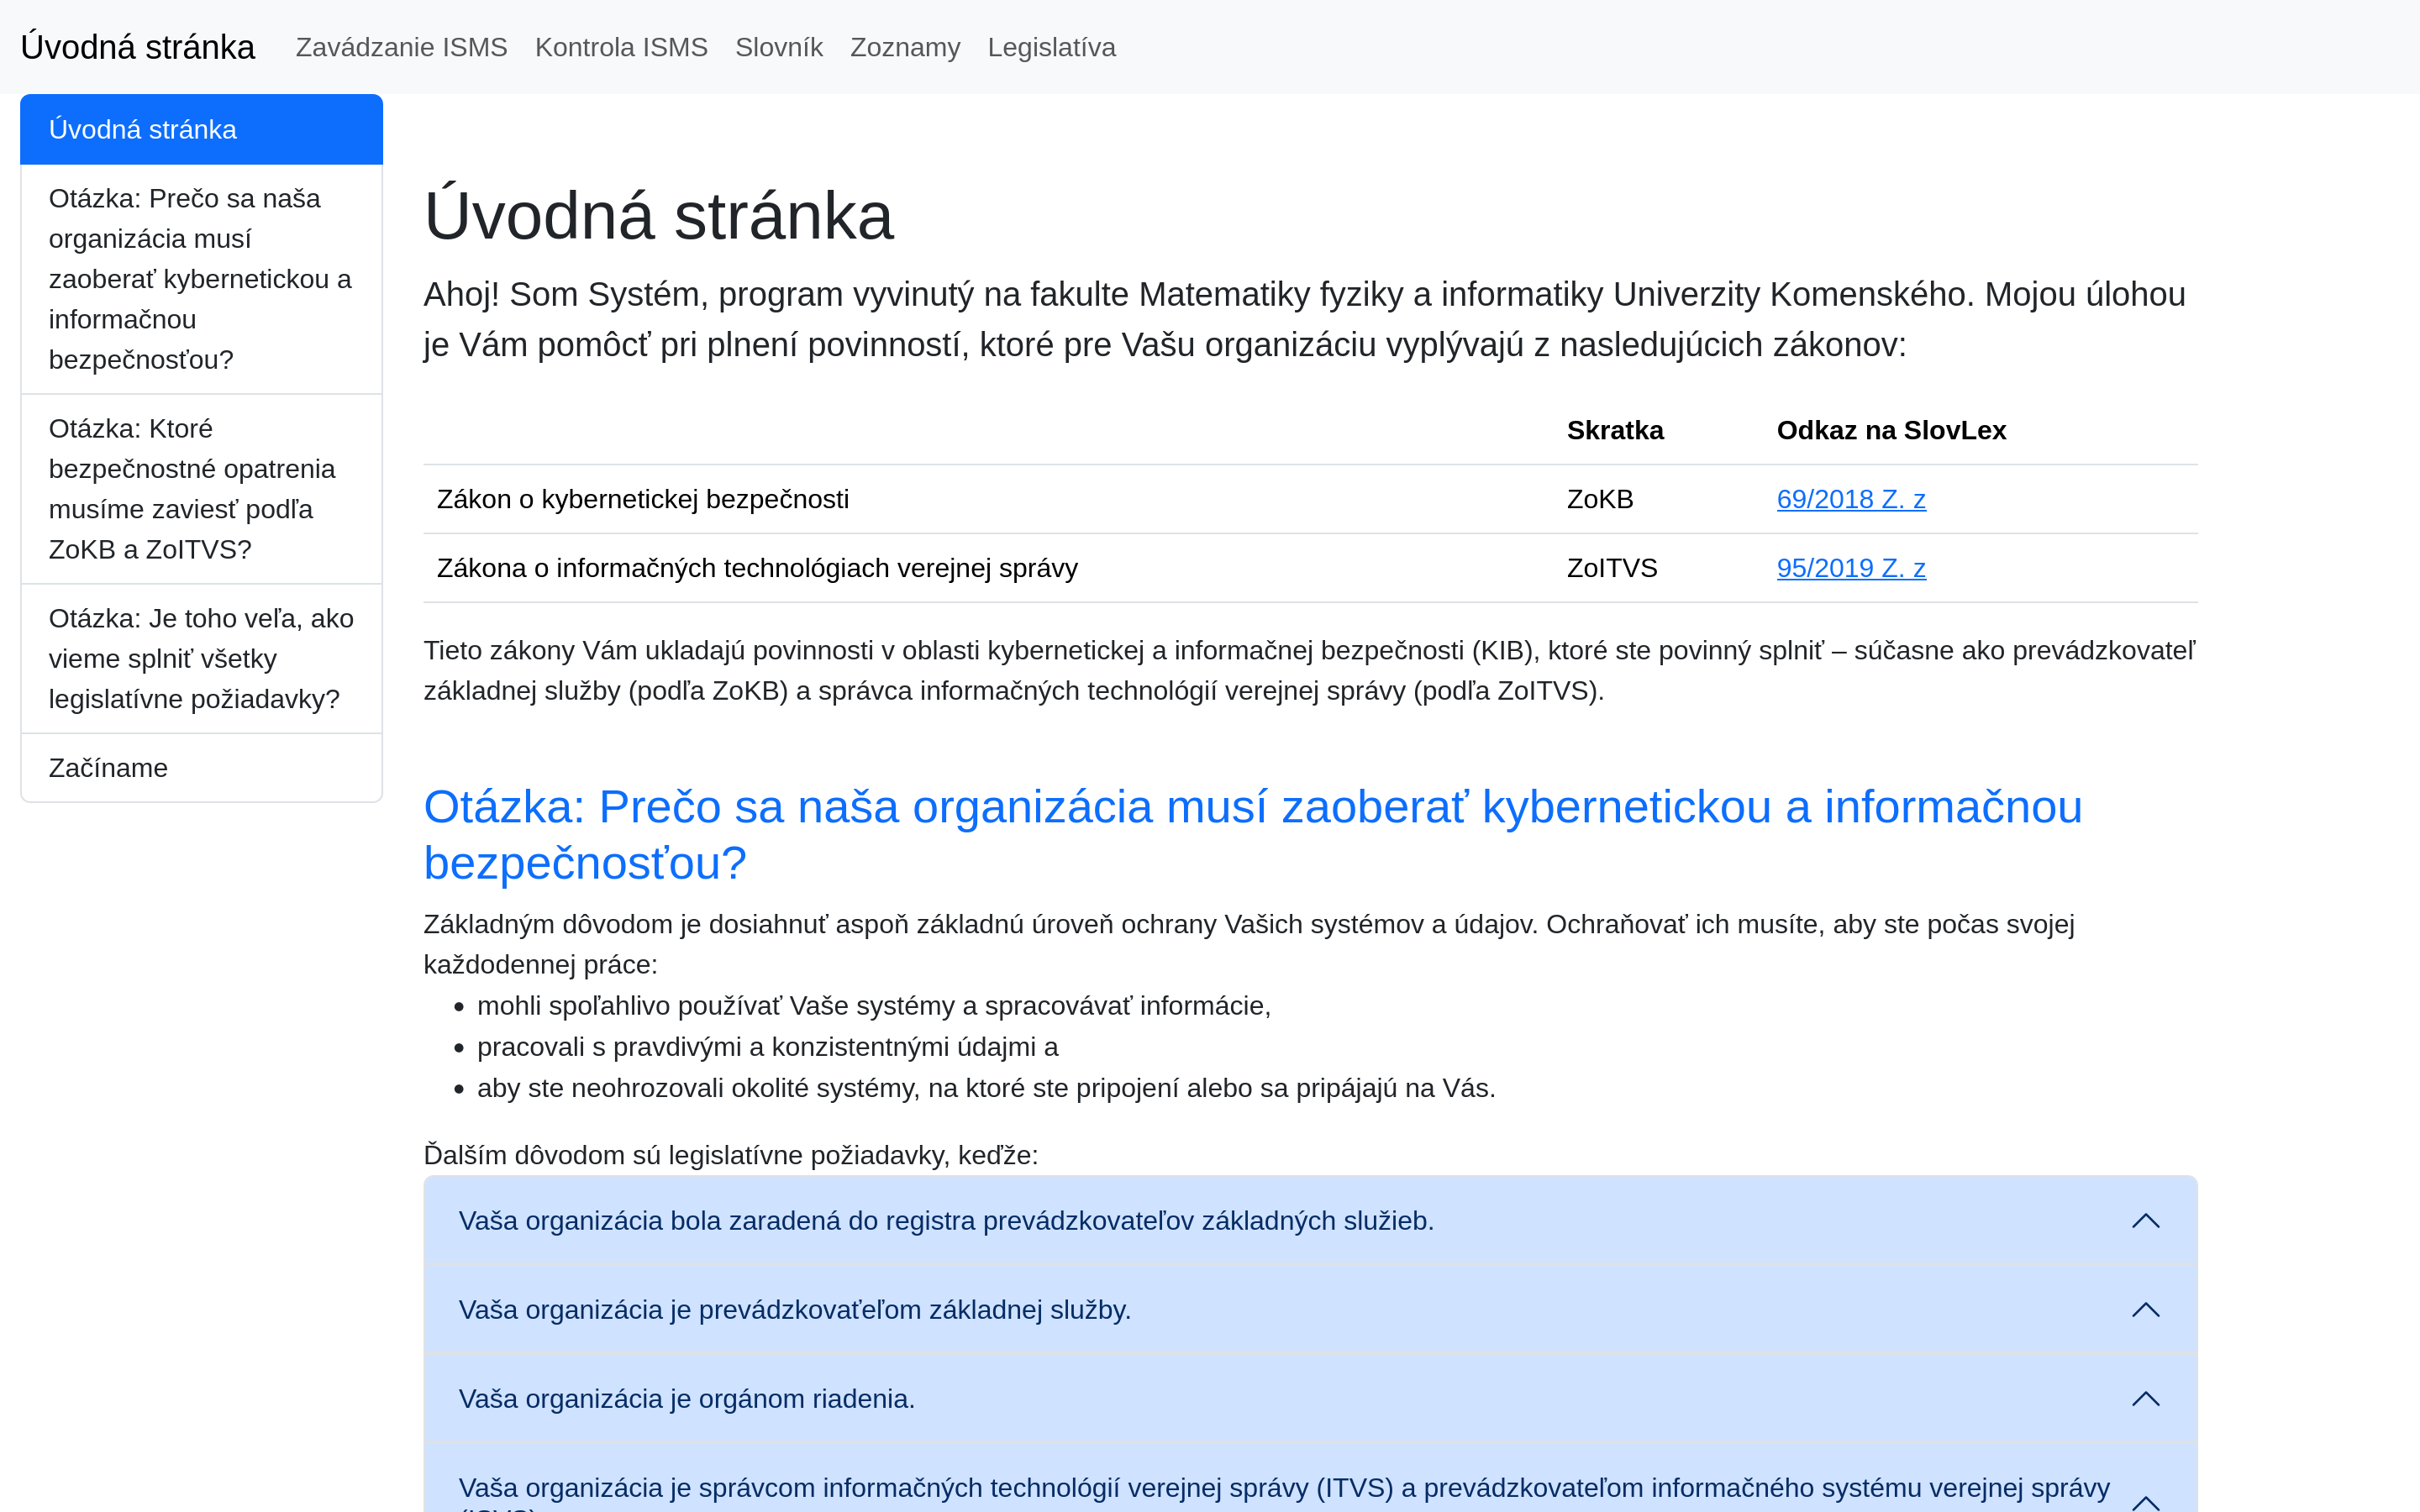
\includegraphics[width=\paperwidth]{images/system-01-uvodna-stranka}}
%  \end{figure}
%\end{frame}
%\begin{frame}
%  \begin{figure}[h]
%    \makebox[\linewidth]{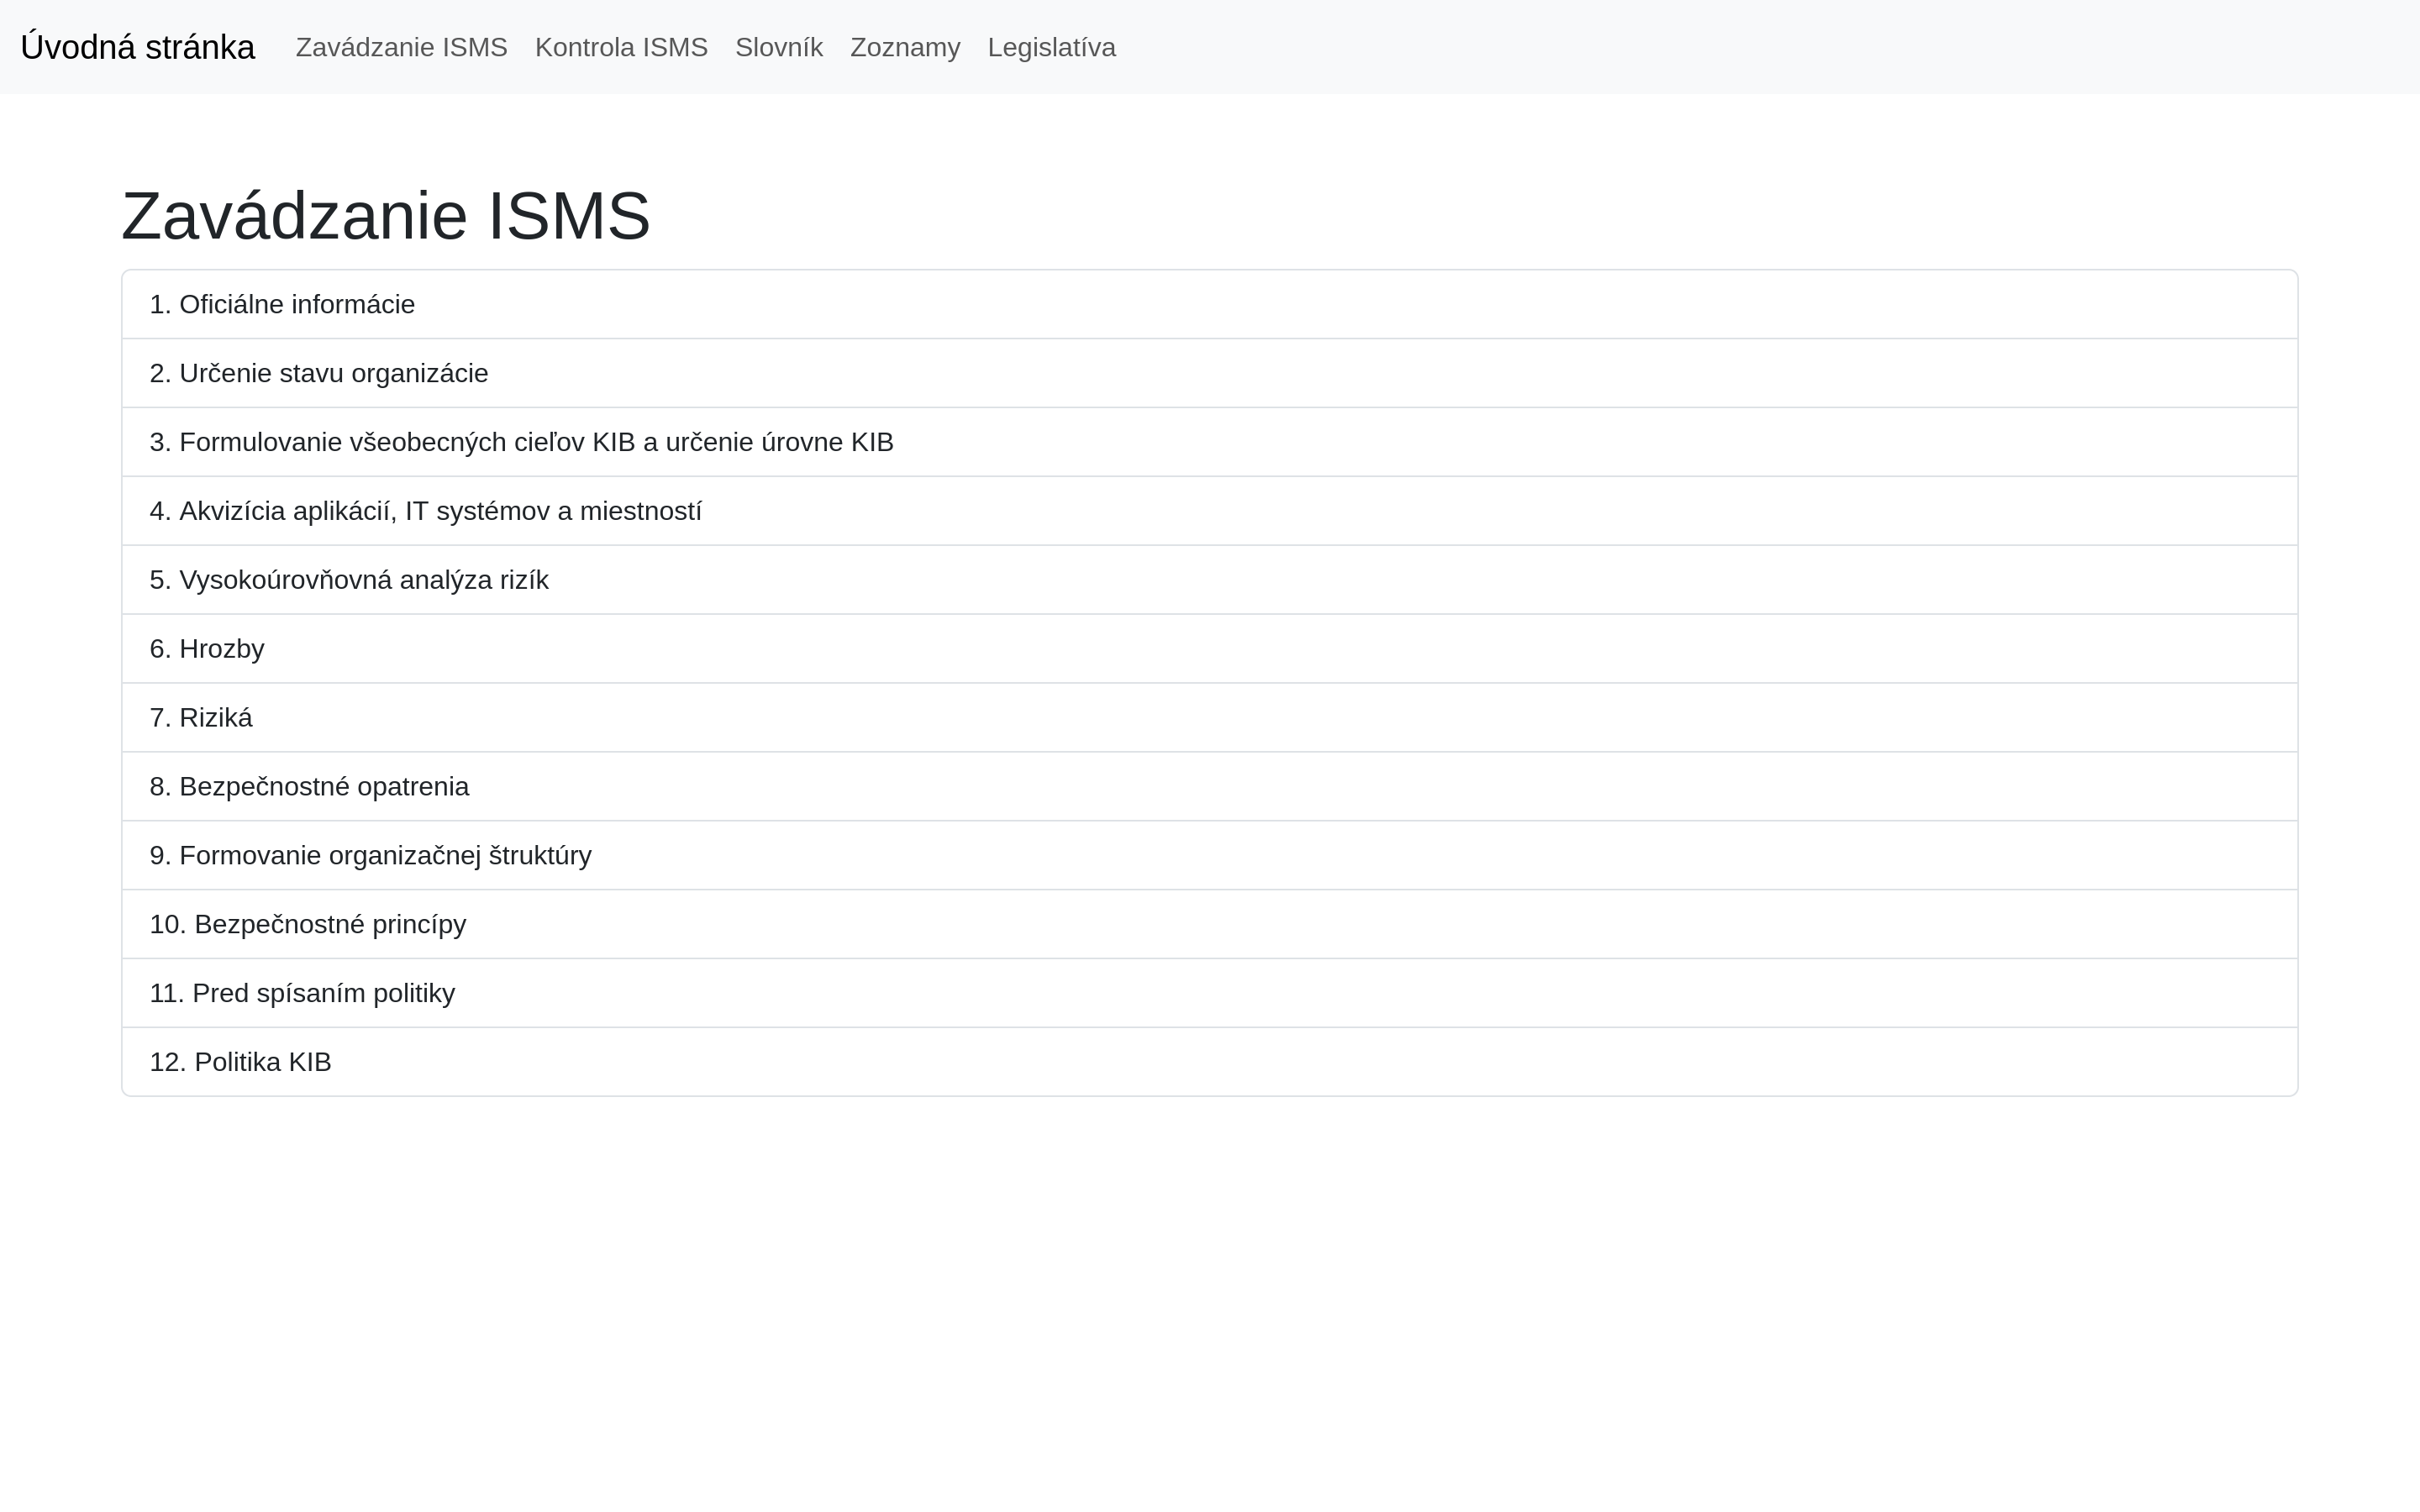
\includegraphics[width=\paperwidth]{images/system-02-zavadzanie-isms}}
%  \end{figure}
%\end{frame}
%\begin{frame}
%  \begin{figure}[h]
%    \makebox[\linewidth]{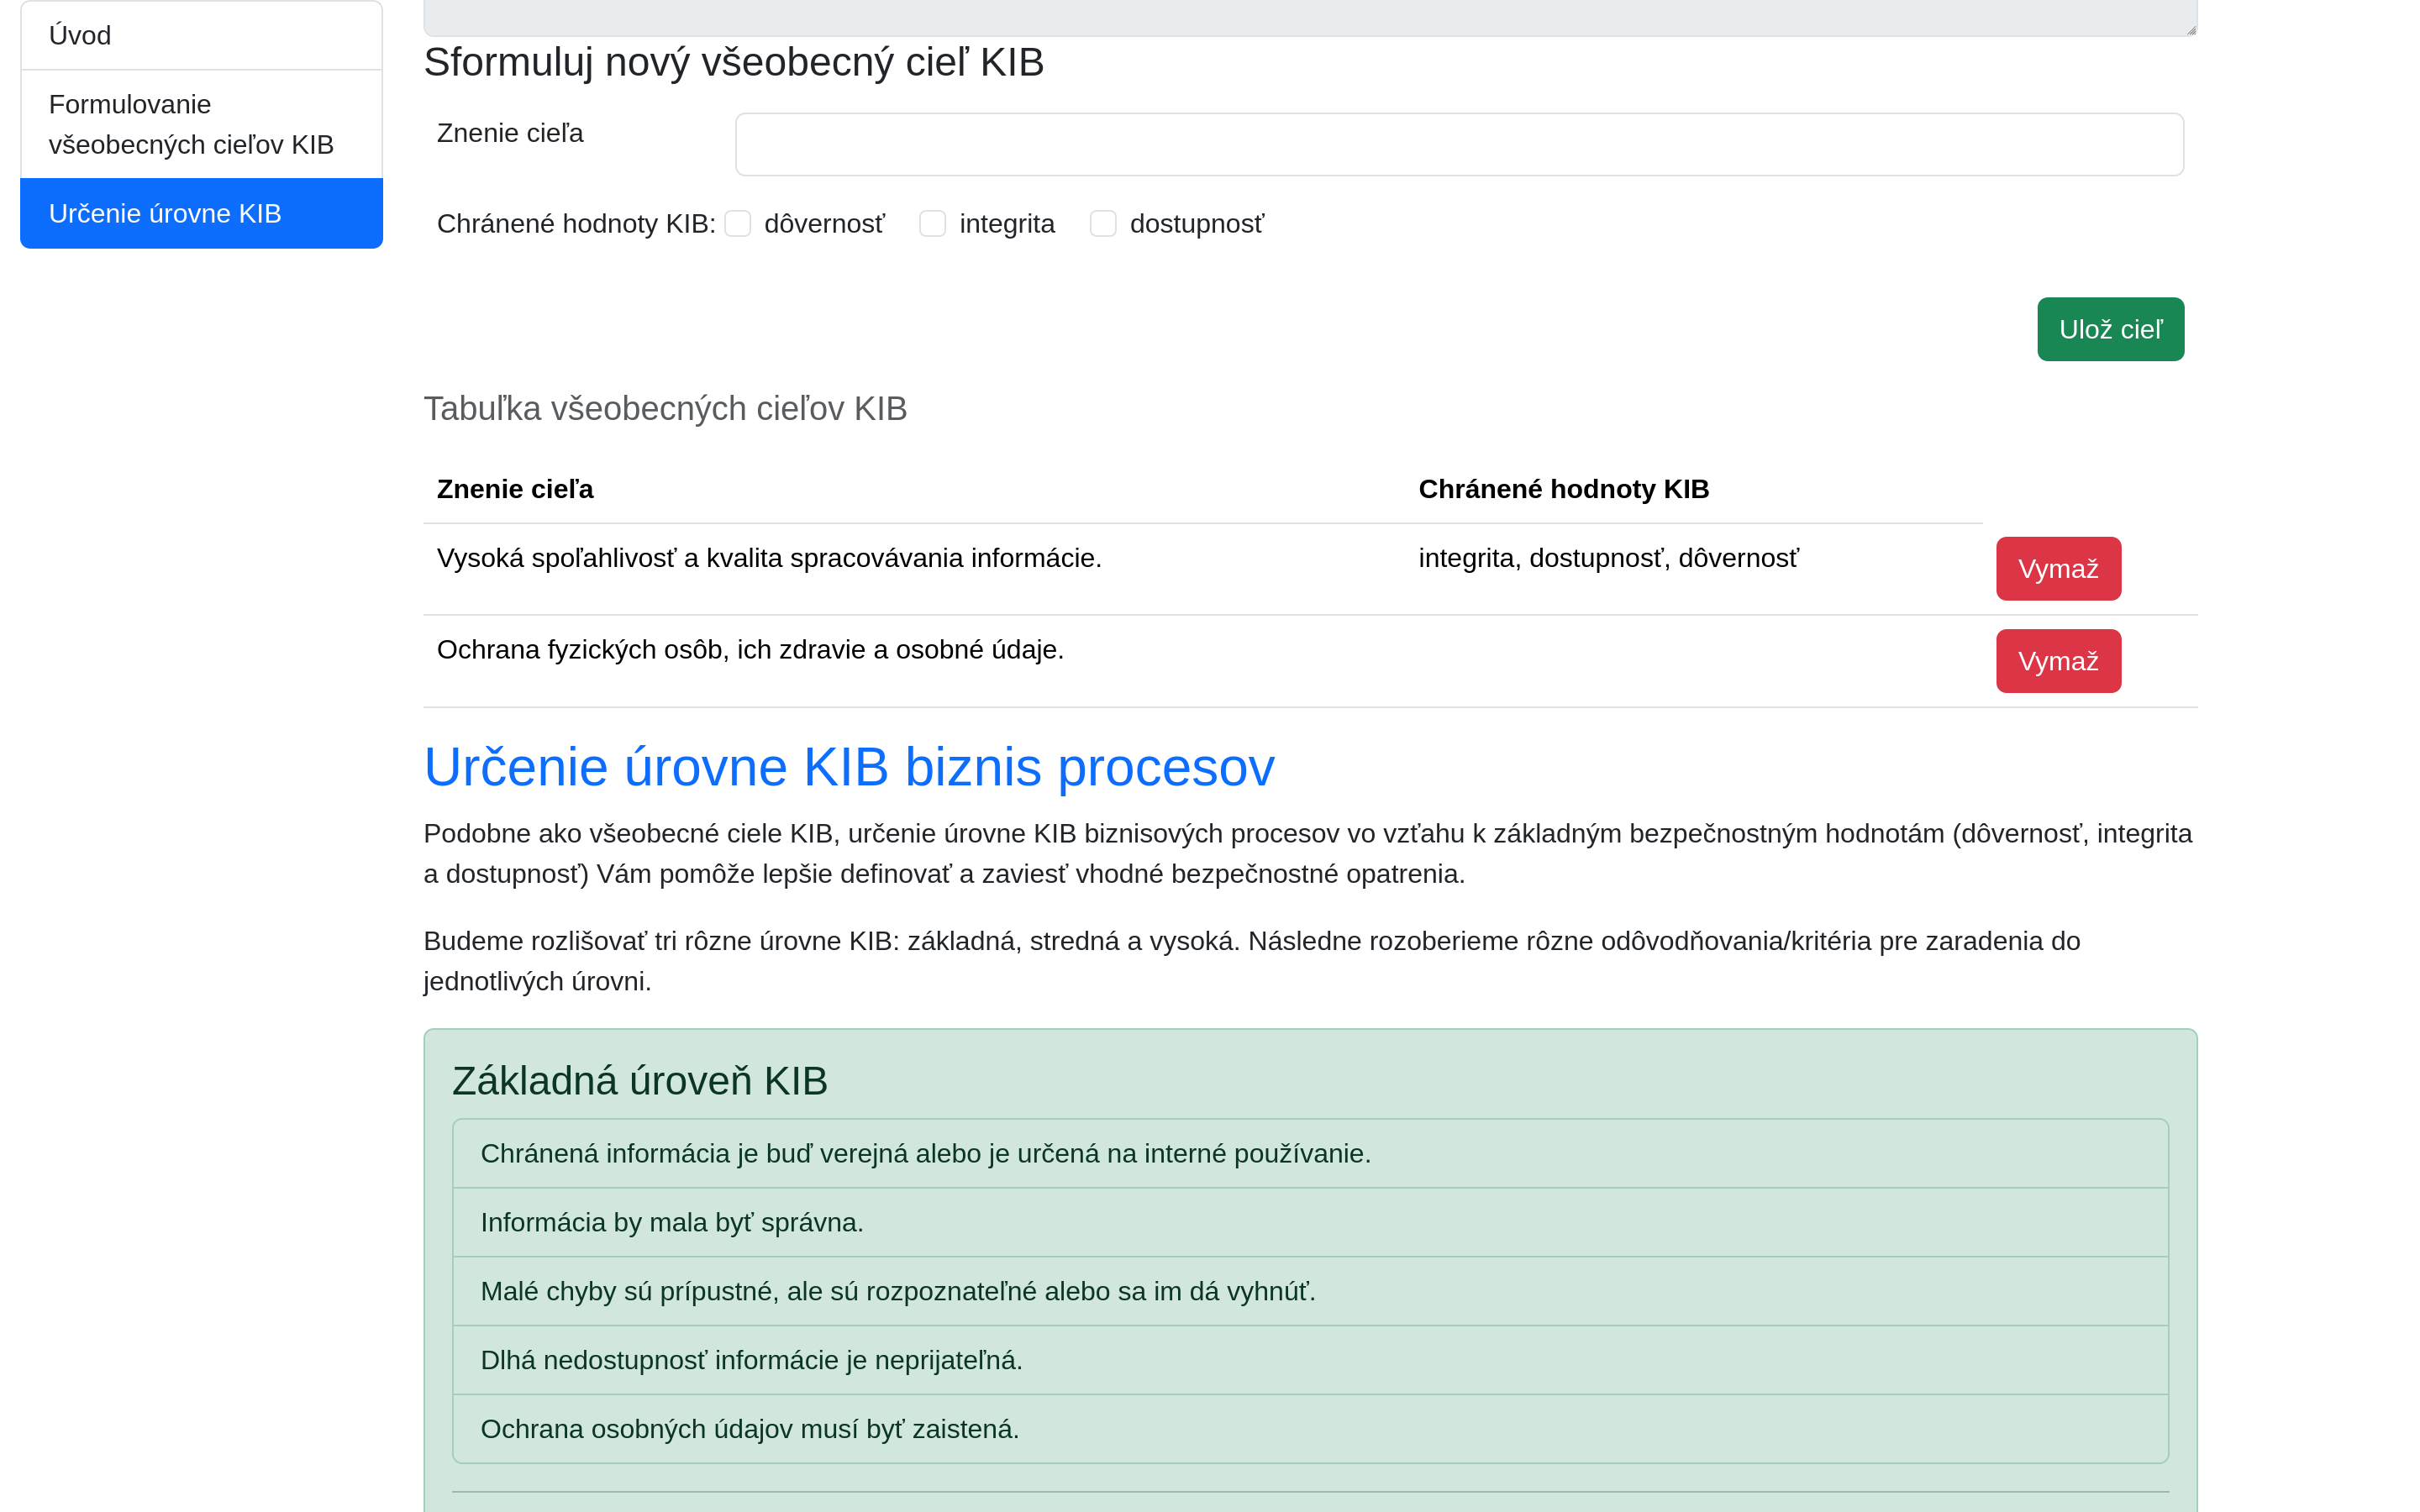
\includegraphics[width=\paperwidth]{images/system-03-formulovanie-cielov}}
%  \end{figure}
%\end{frame}
%\begin{frame}
%  \begin{figure}[h]
%    \makebox[\linewidth]{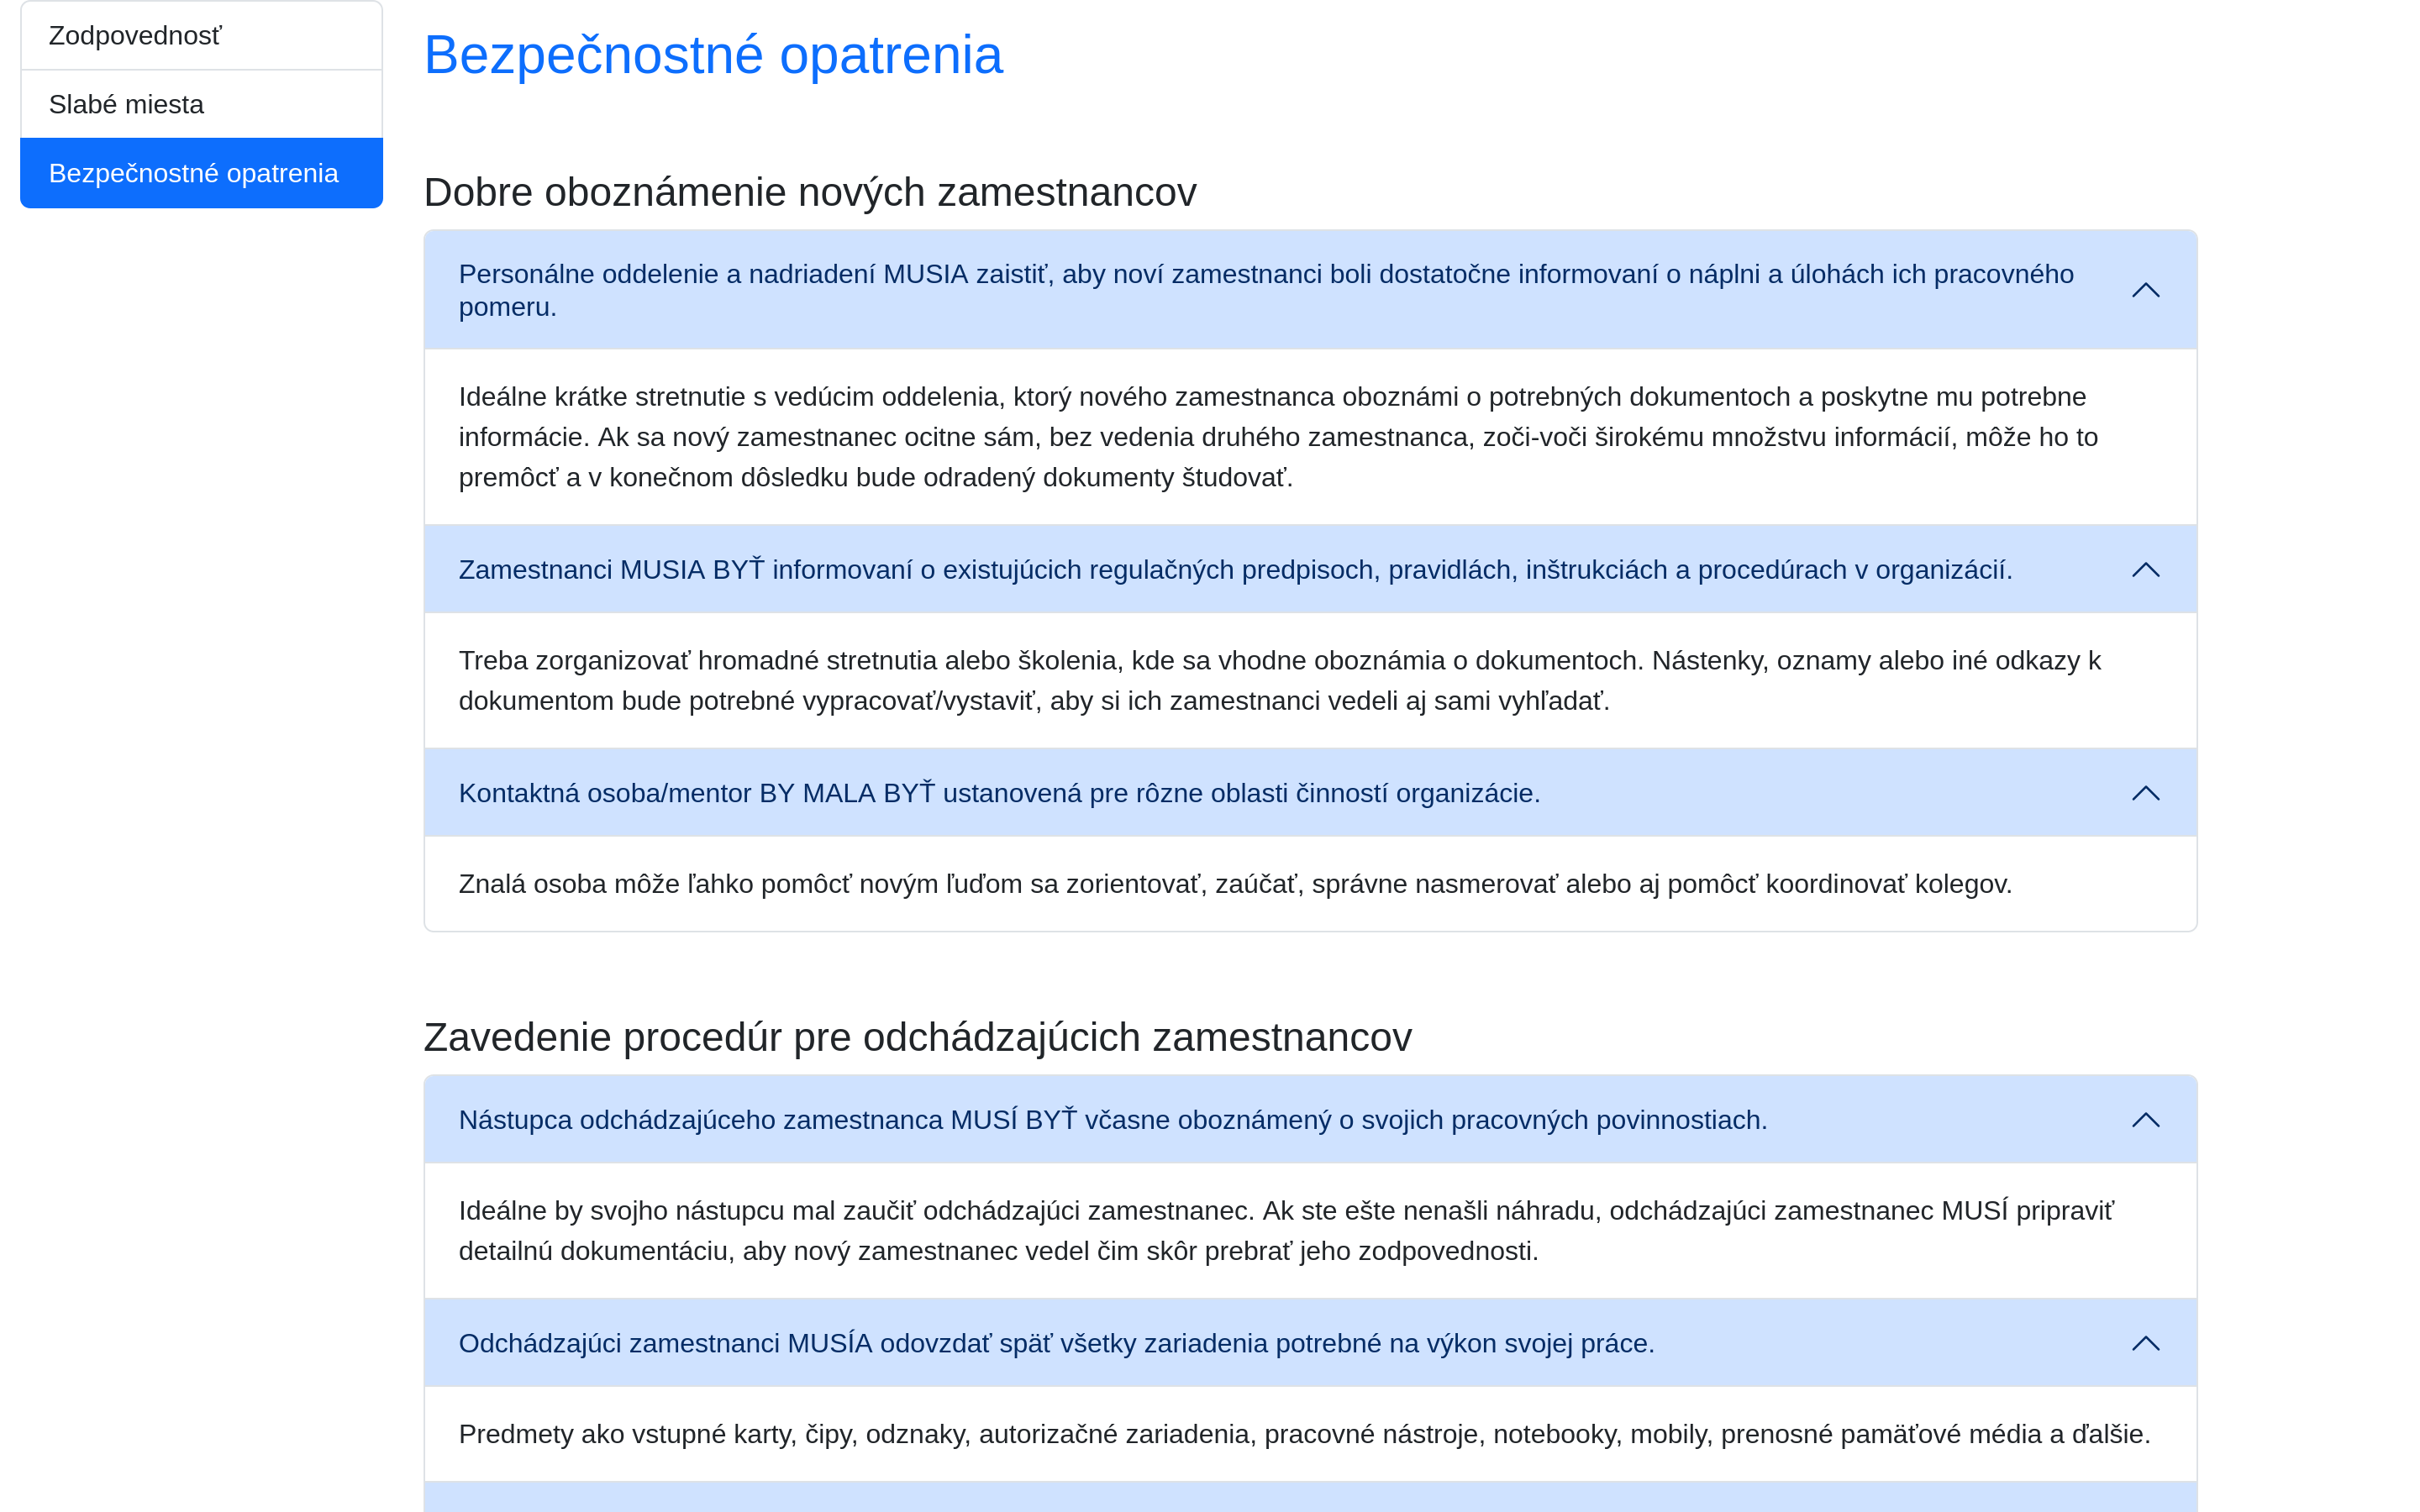
\includegraphics[width=\paperwidth]{images/system-04-bezpecnostne-opatrenia}}
%  \end{figure}
%\end{frame}
%\begin{frame}
%  \begin{figure}[h]
%    \makebox[\linewidth]{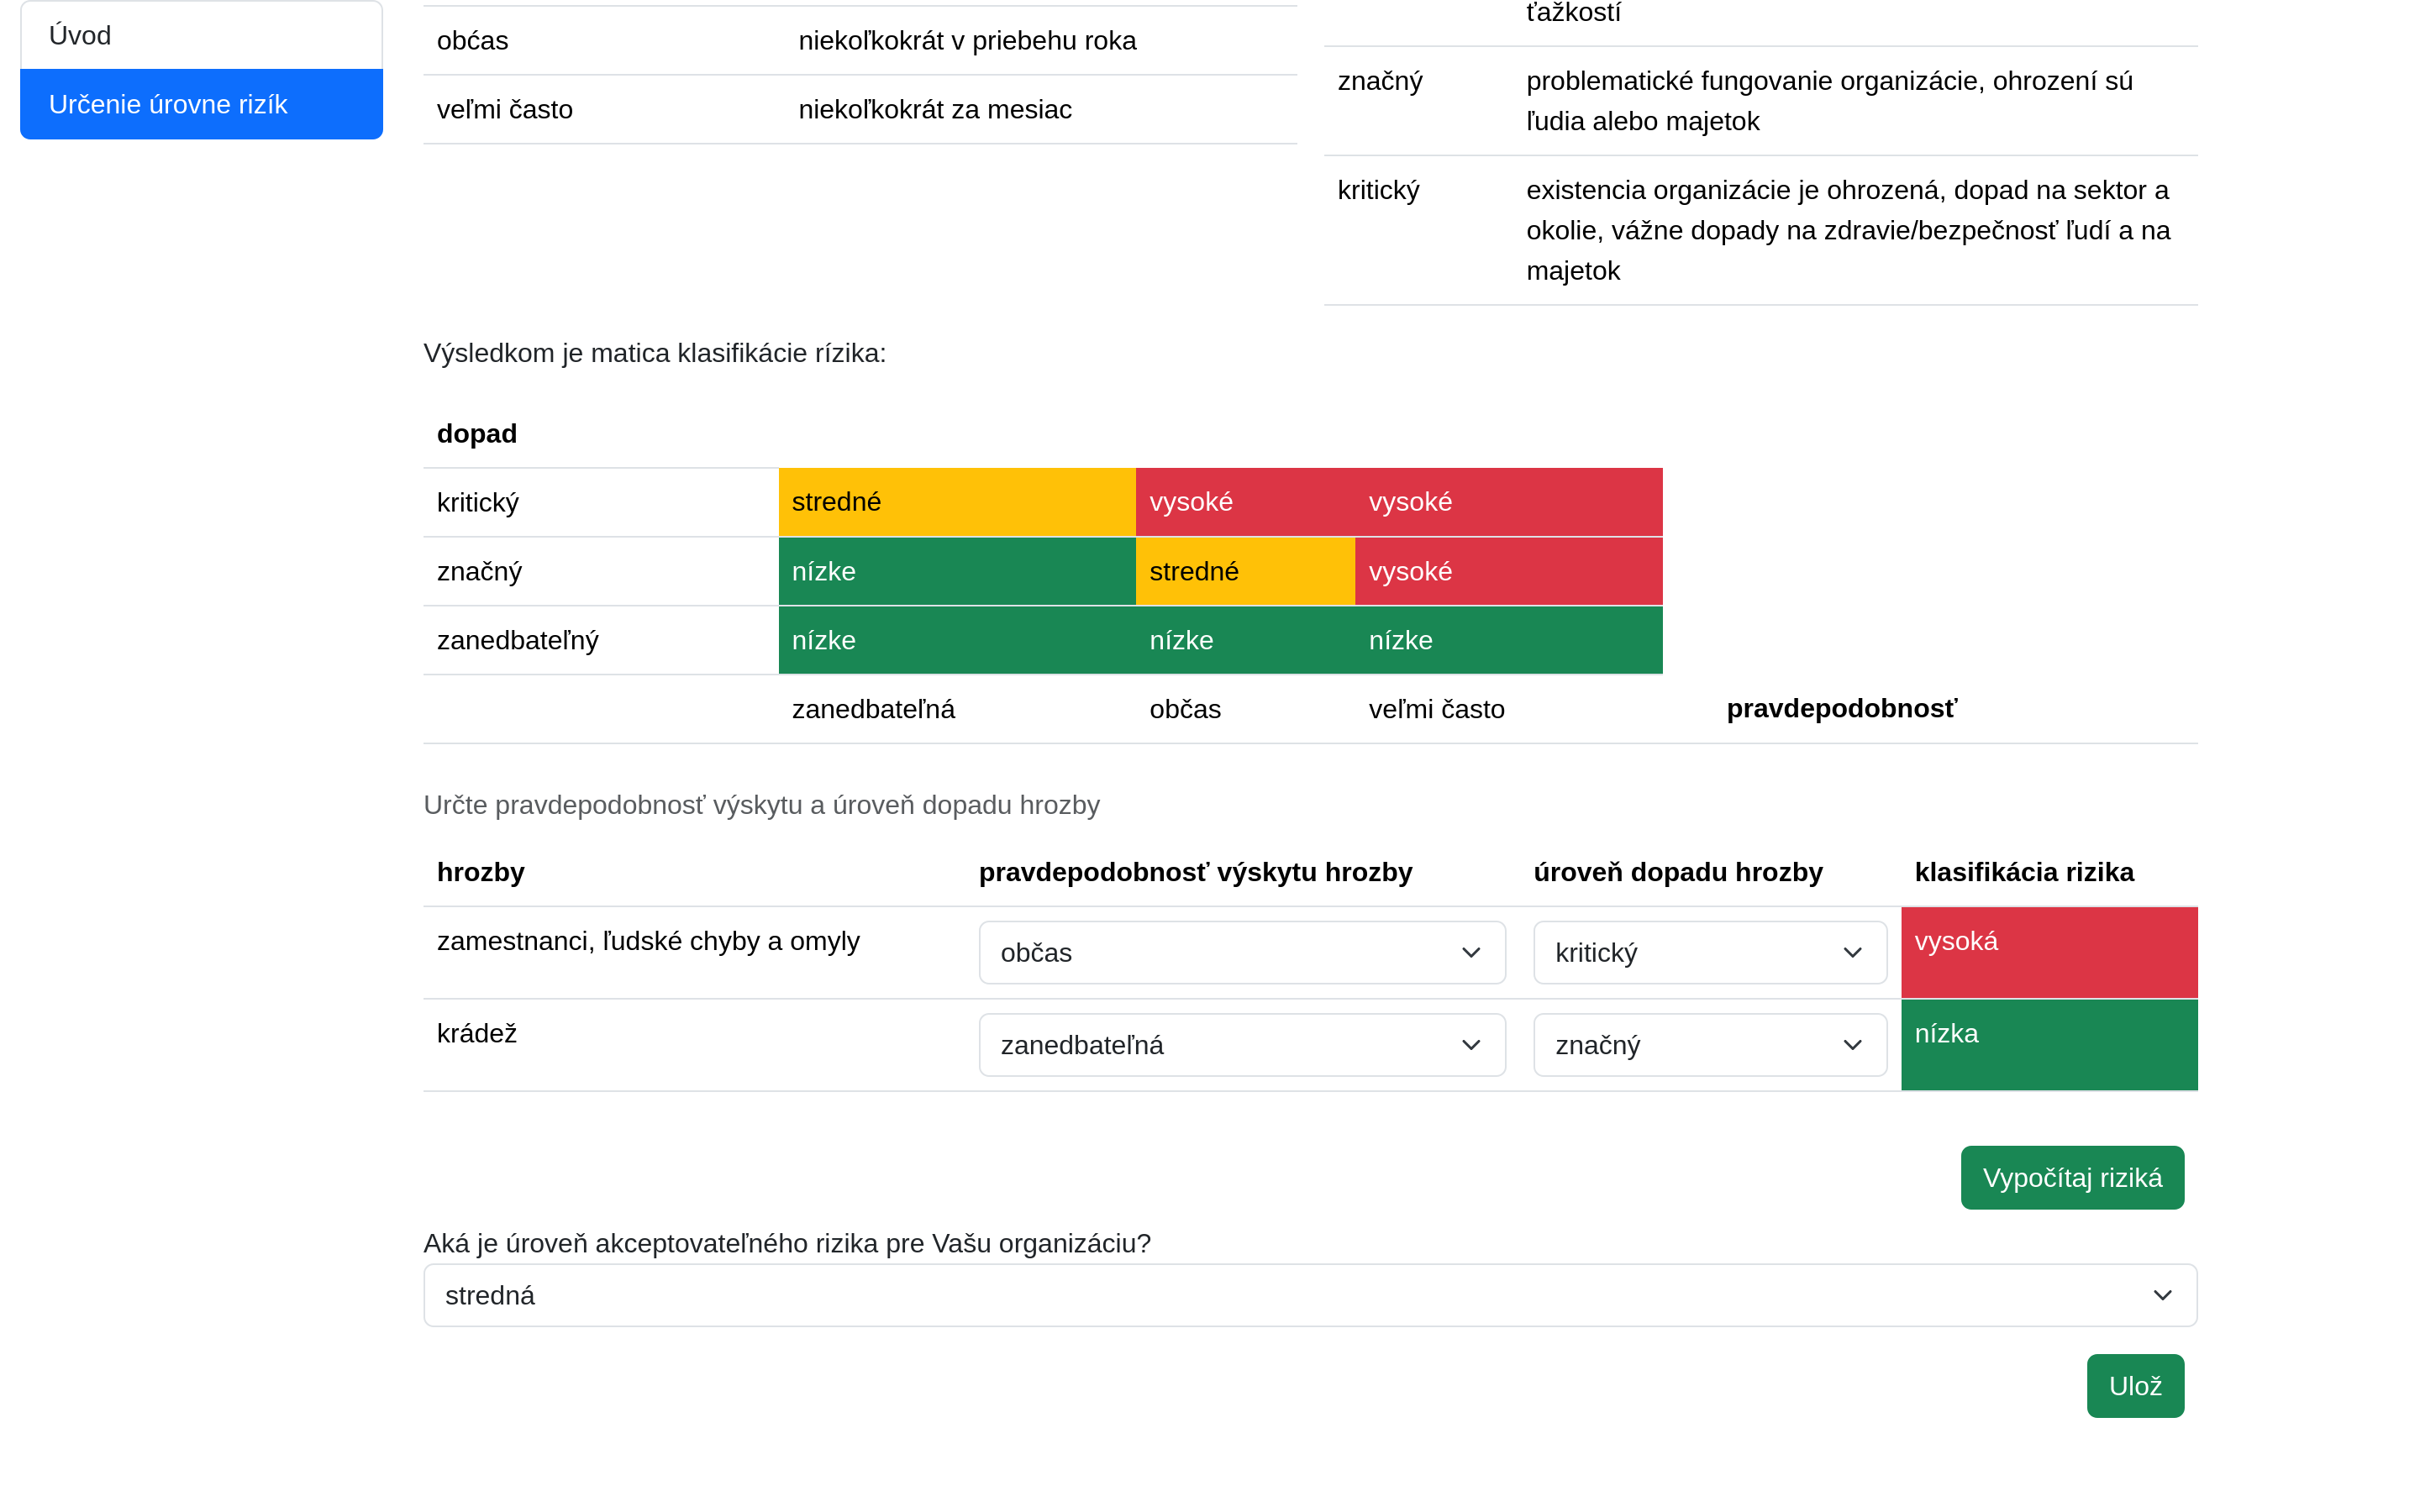
\includegraphics[width=\paperwidth]{images/system-05-rizika}}
%  \end{figure}
%\end{frame}
%\begin{frame}
%  \begin{figure}[h]
%    \makebox[\linewidth]{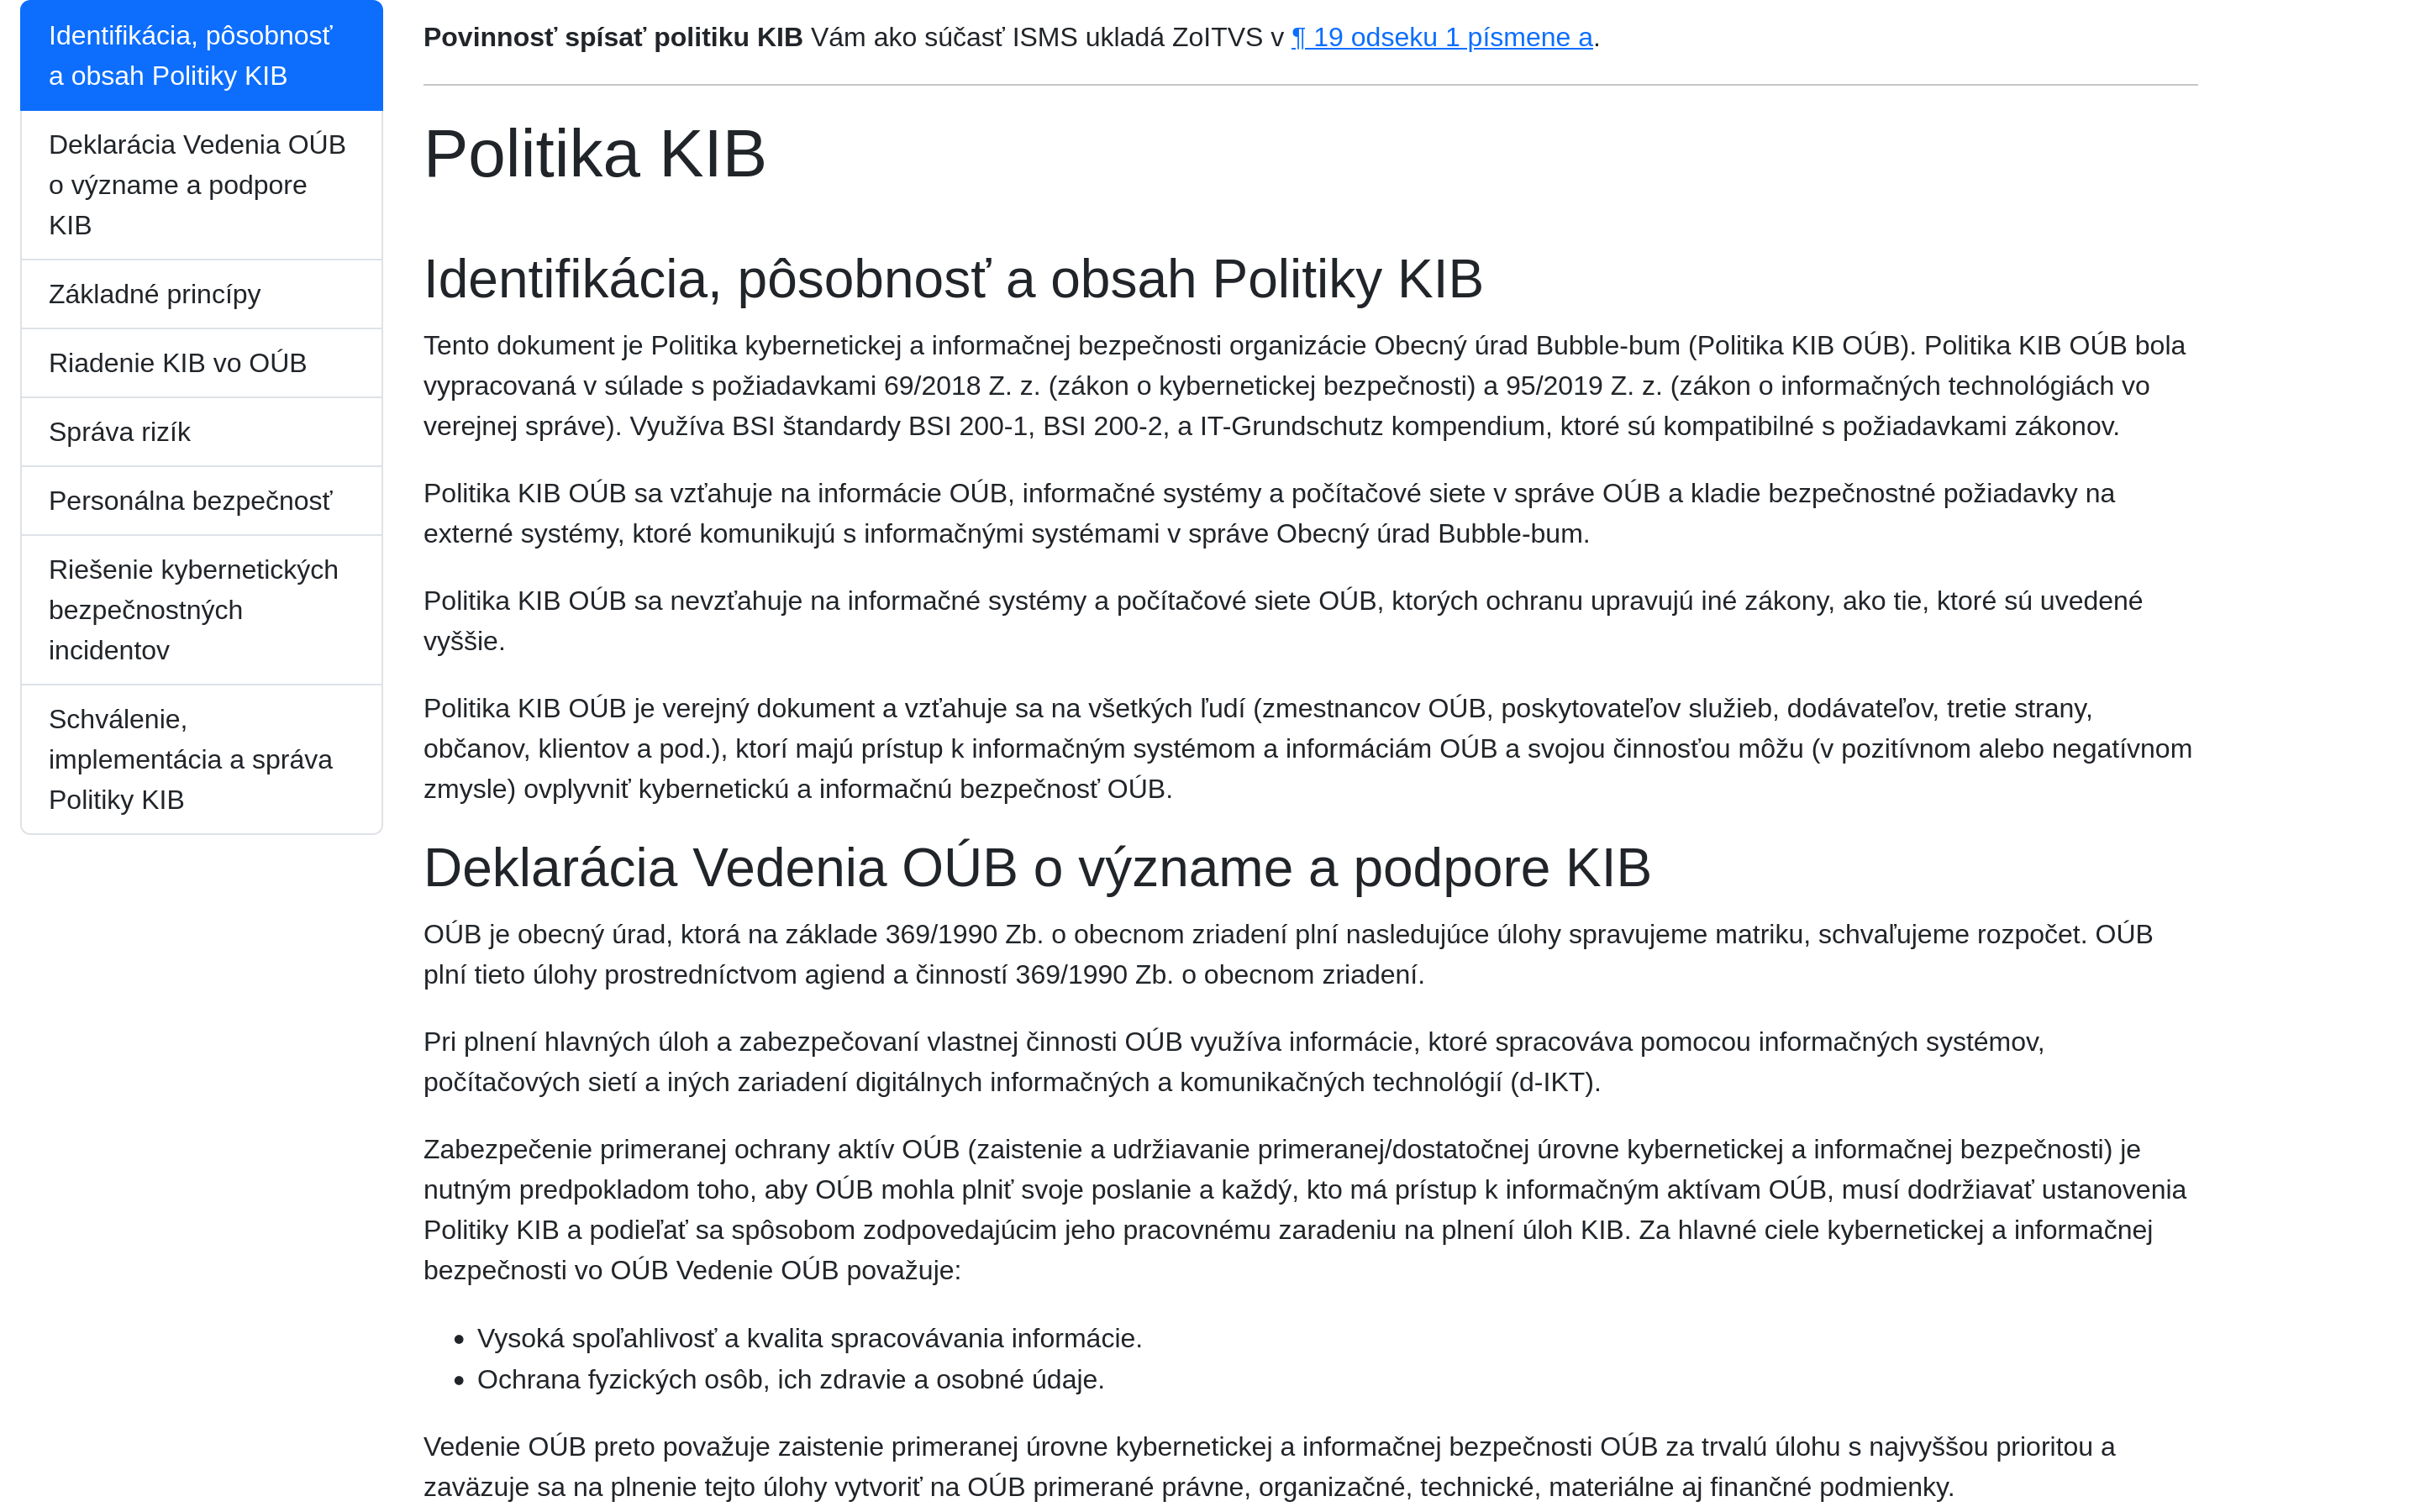
\includegraphics[width=\paperwidth]{images/system-06-politika}}
%  \end{figure}
%\end{frame}
%\begin{frame}
%  \begin{figure}[h]
%    \makebox[\linewidth]{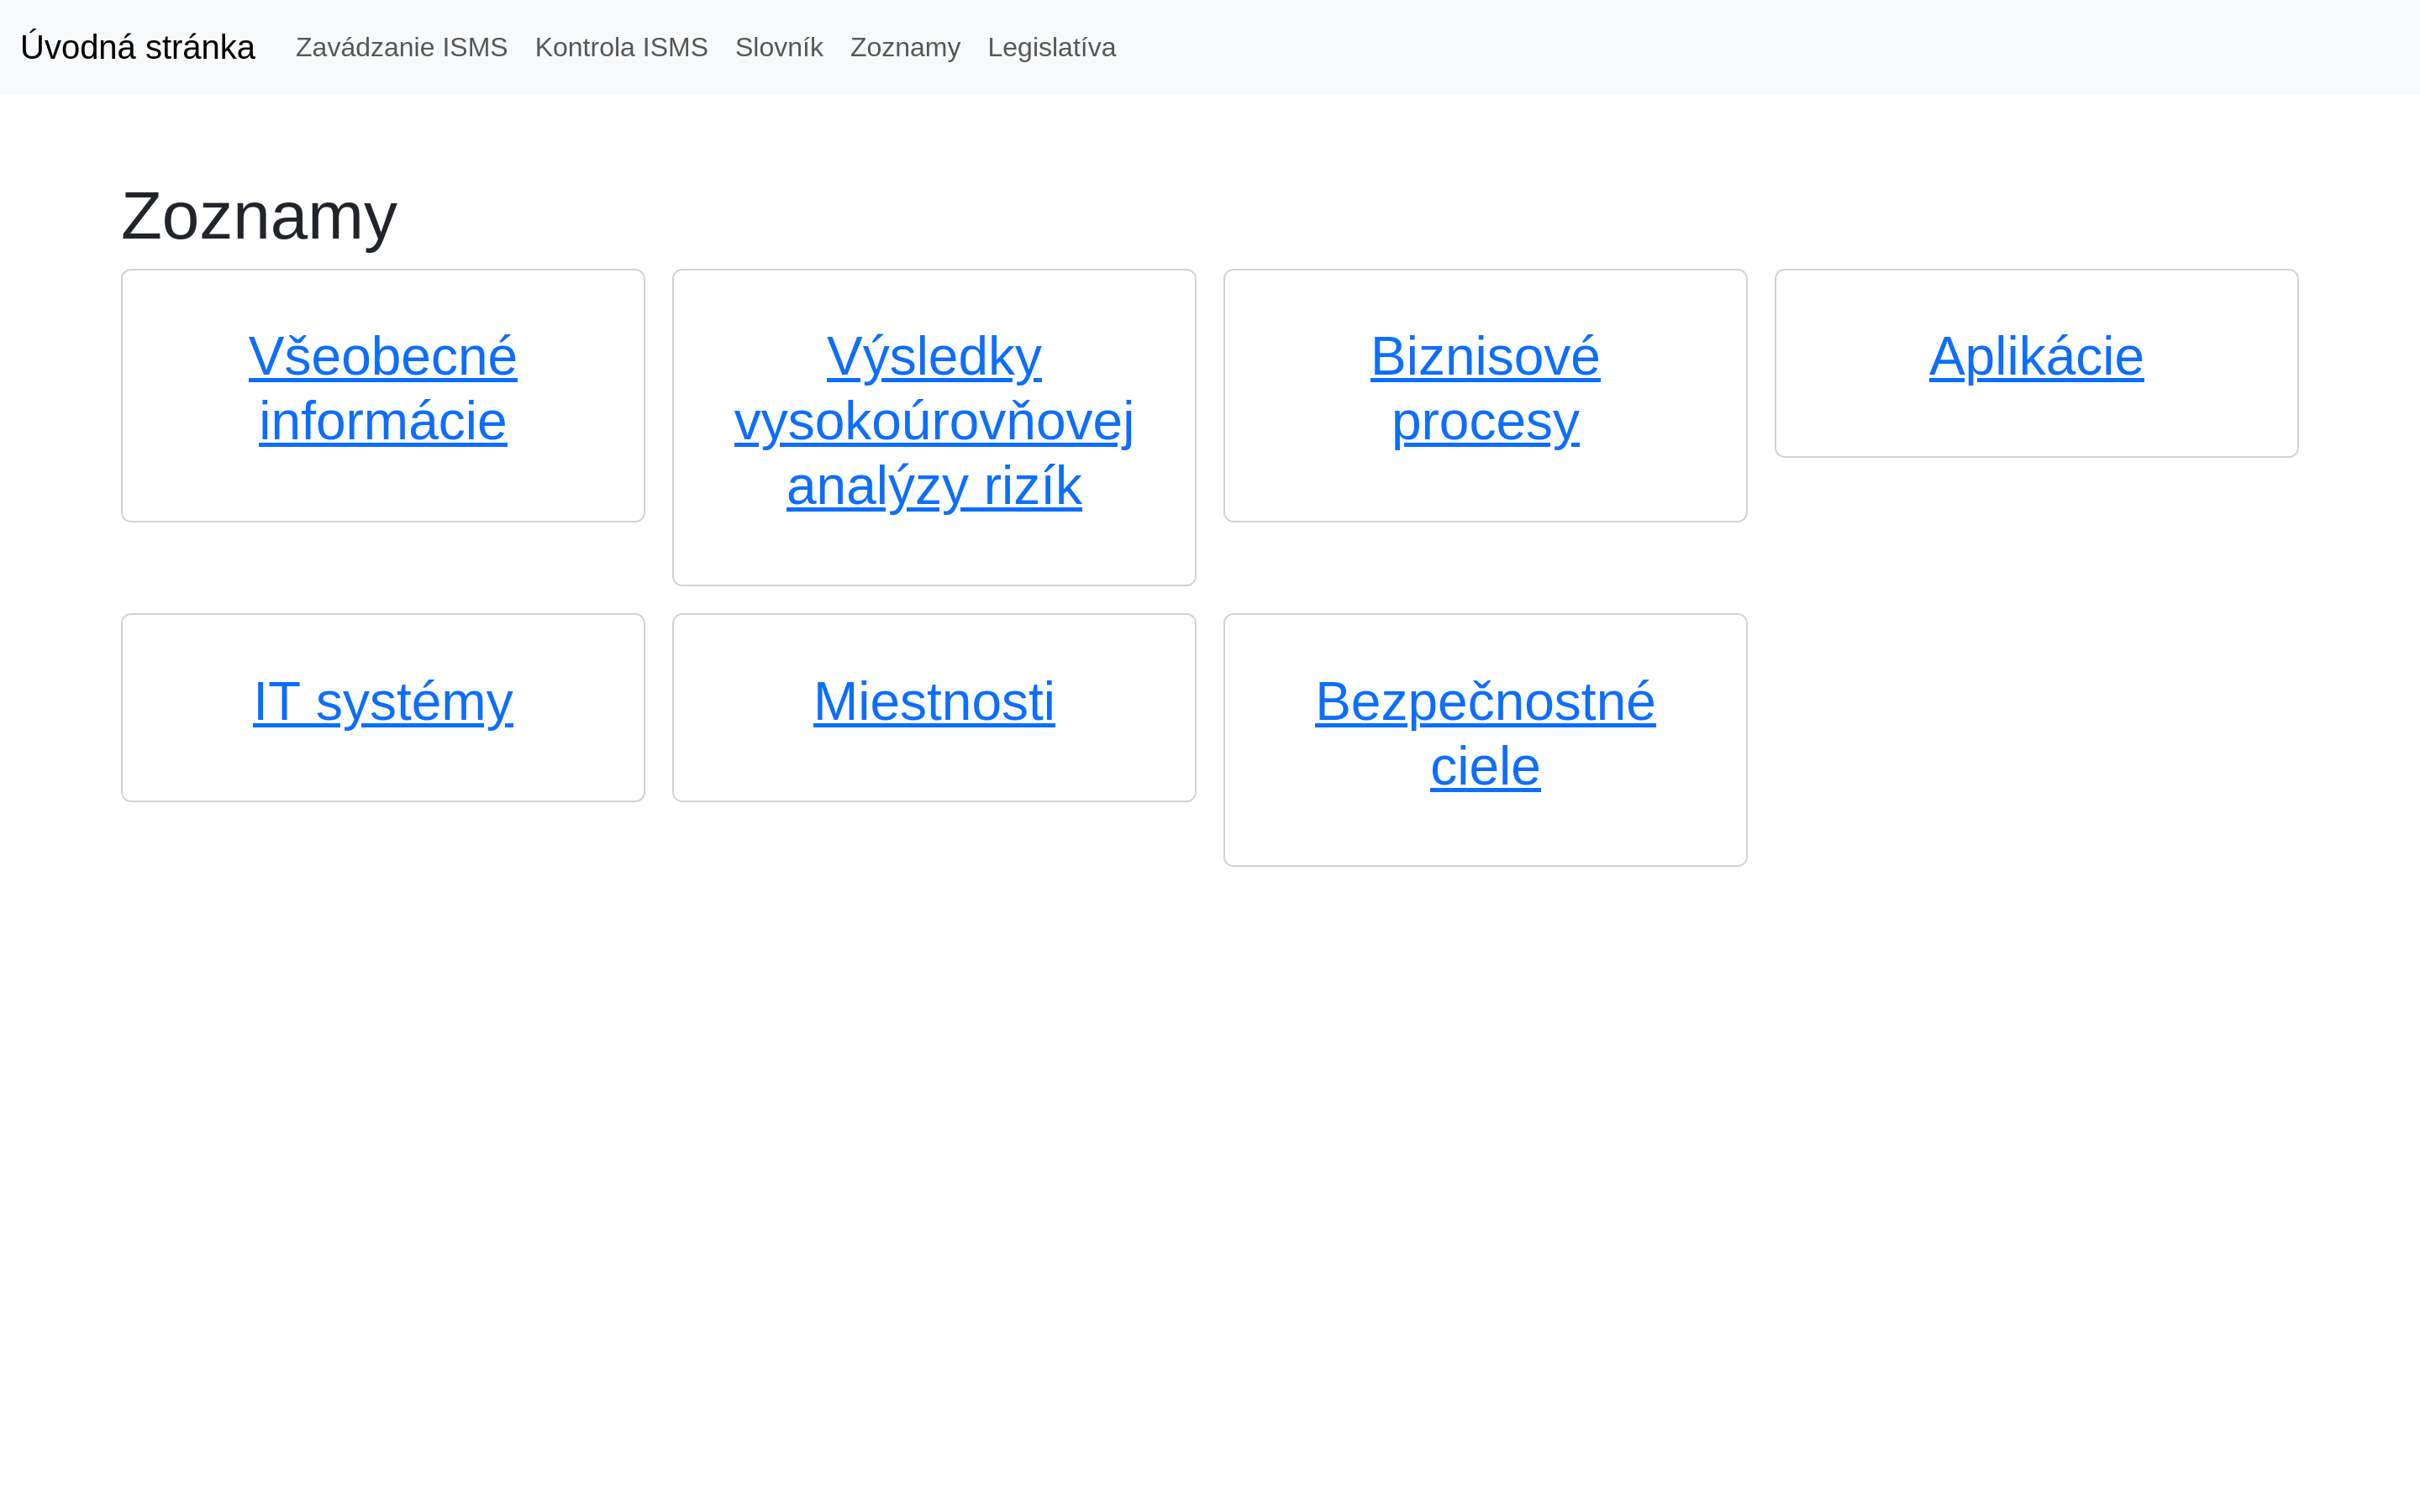
\includegraphics[width=\paperwidth]{images/system-07-zoznamy.png}}
%  \end{figure}
%\end{frame}
%\begin{frame}
%  \begin{figure}[h]
%    \makebox[\linewidth]{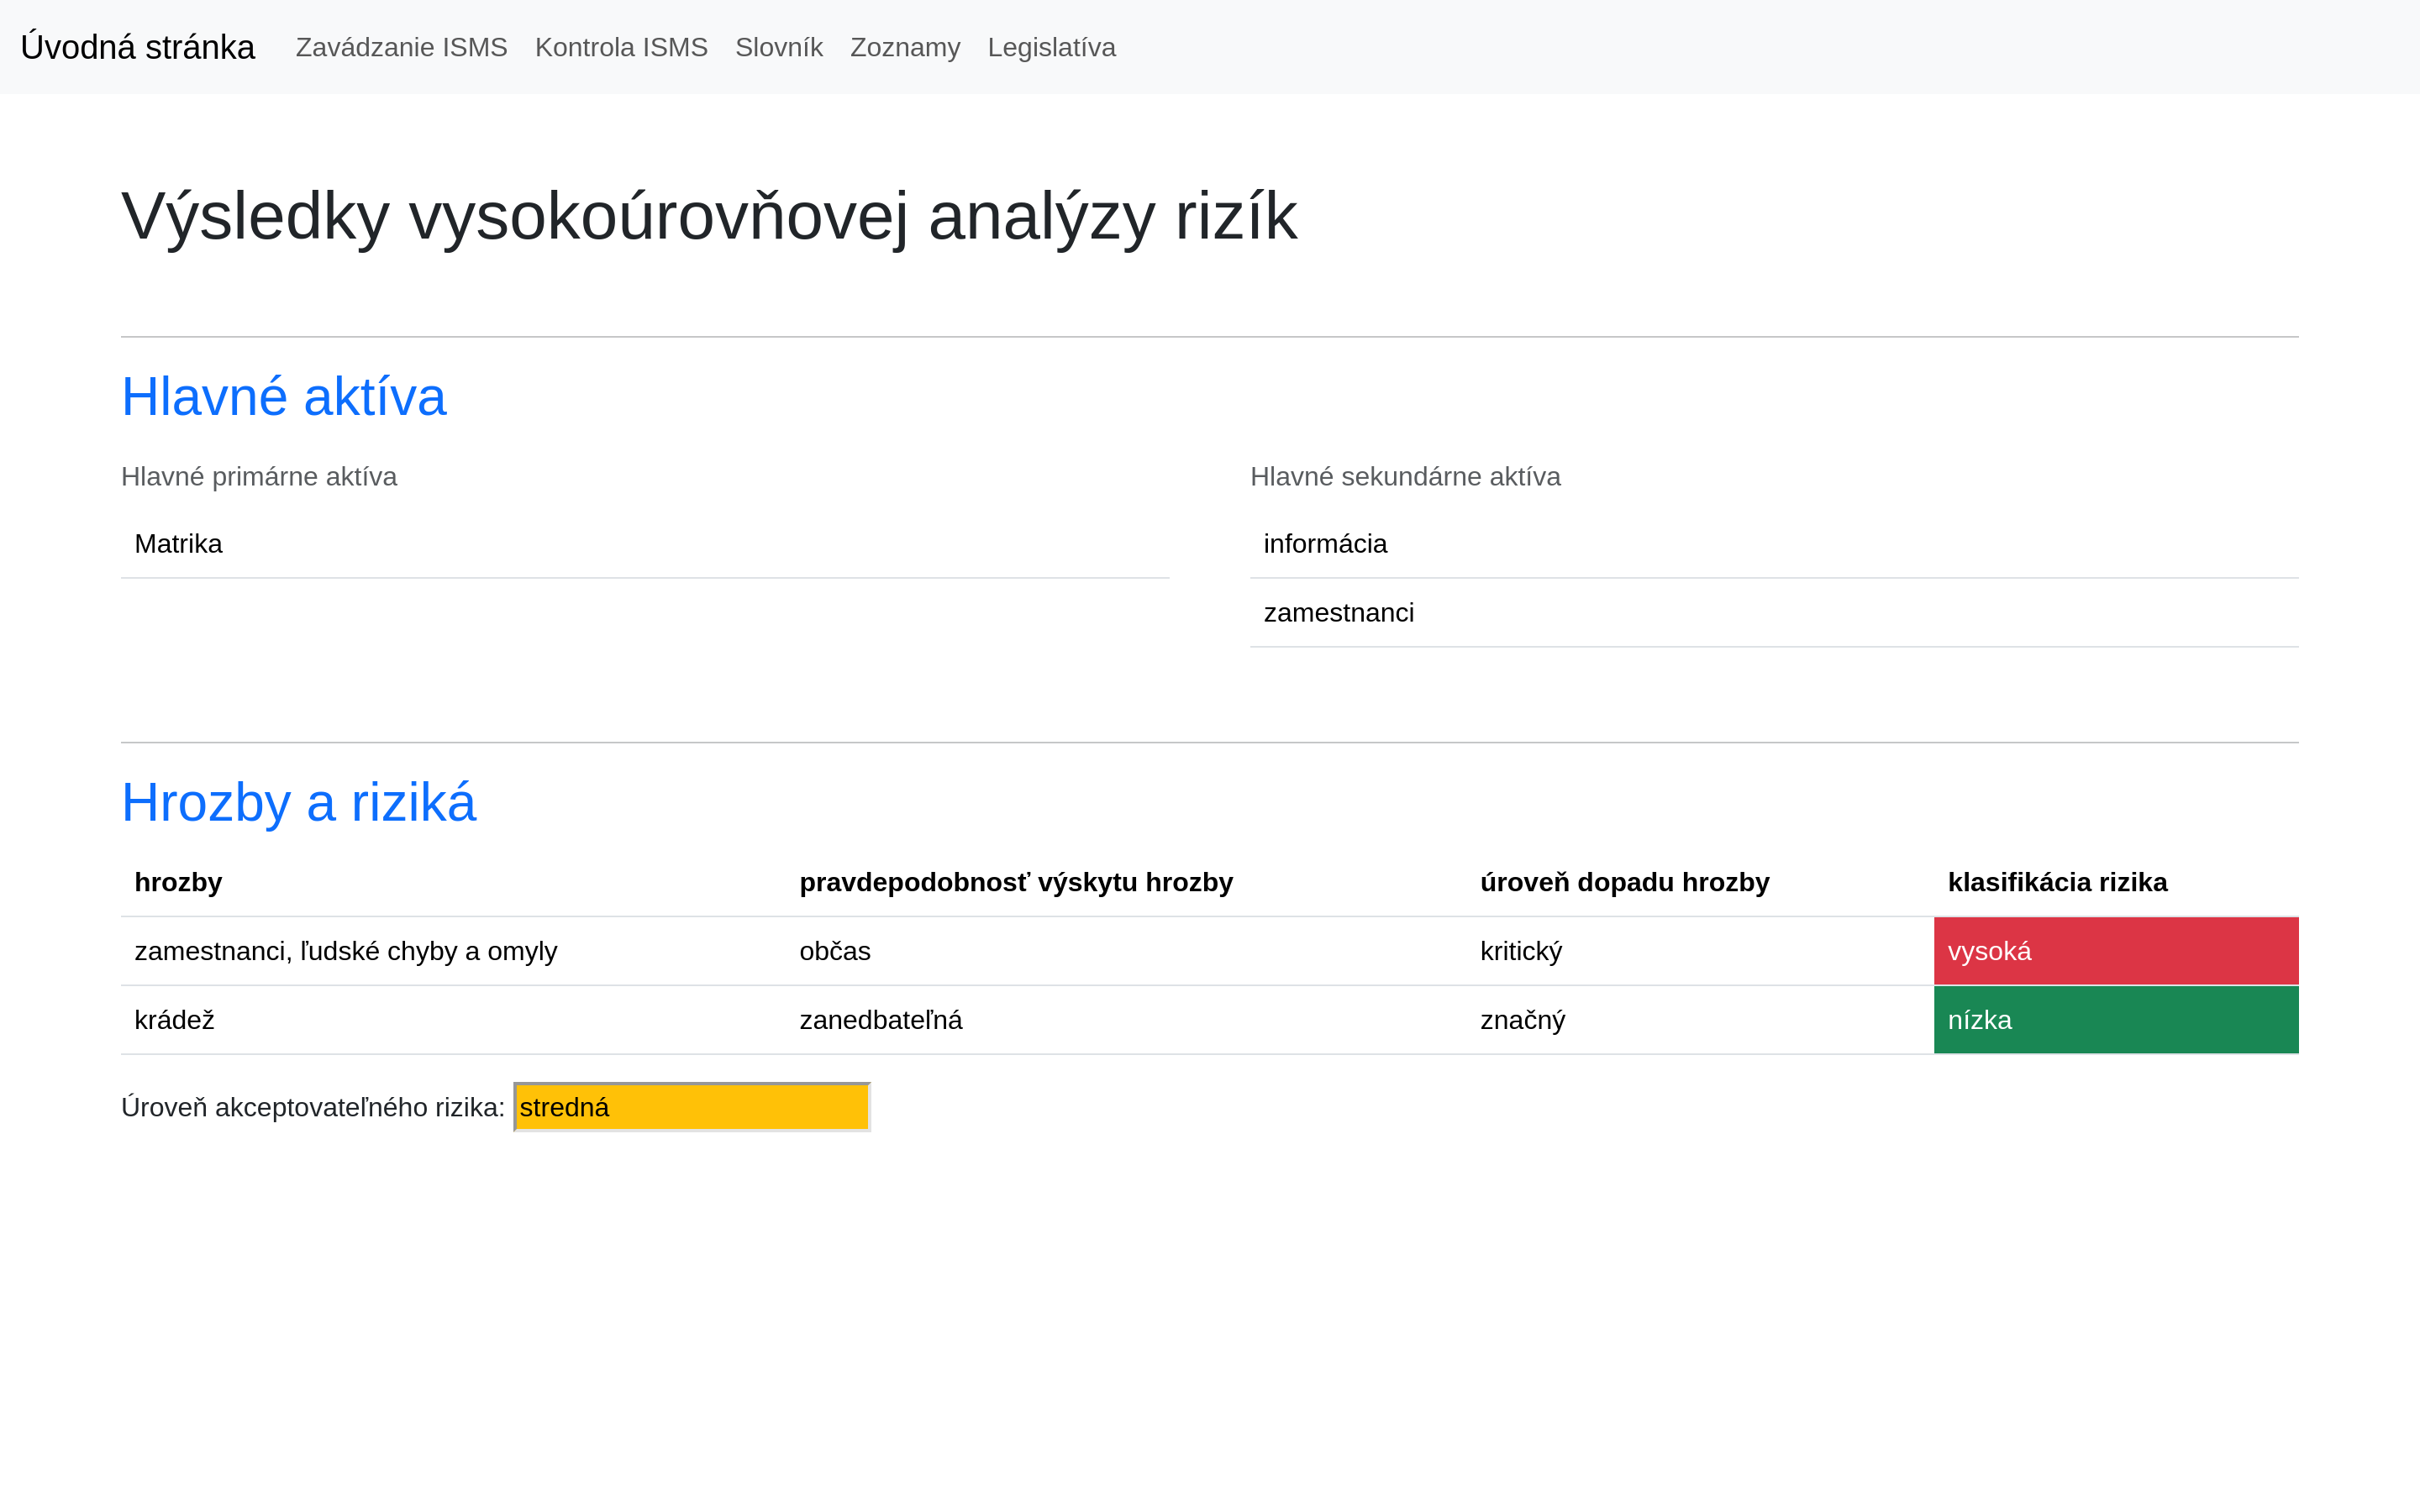
\includegraphics[width=\paperwidth]{images/system-08-zoznam-vysokourovnova-analyza-rizik.png}}
%  \end{figure}
%\end{frame}

\begin{frame}
  \frametitle{Datábazový pohľad}
    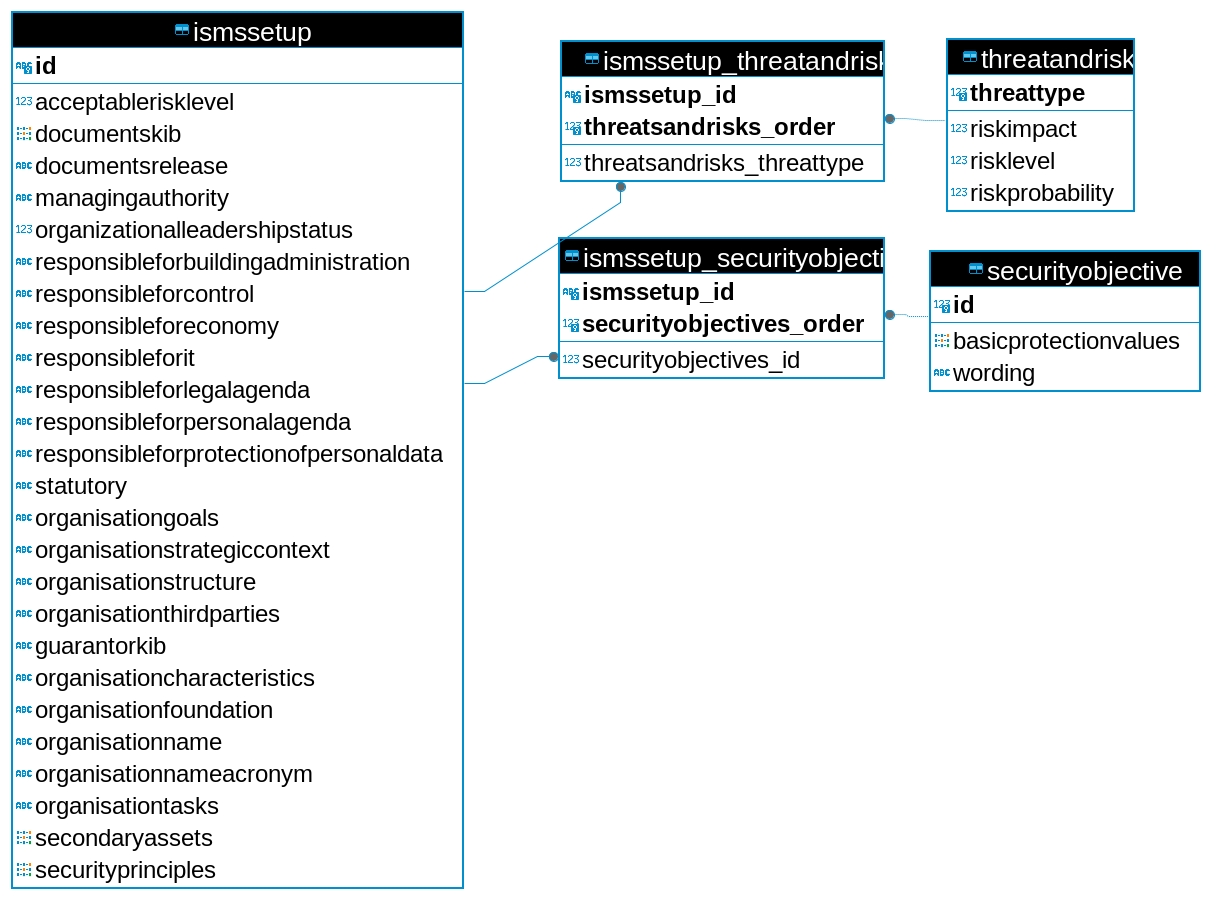
\includegraphics[width=9cm]{images/database-diagram-isms-setup}
\end{frame}
\begin{frame}
  \frametitle{Datábazový pohľad}
    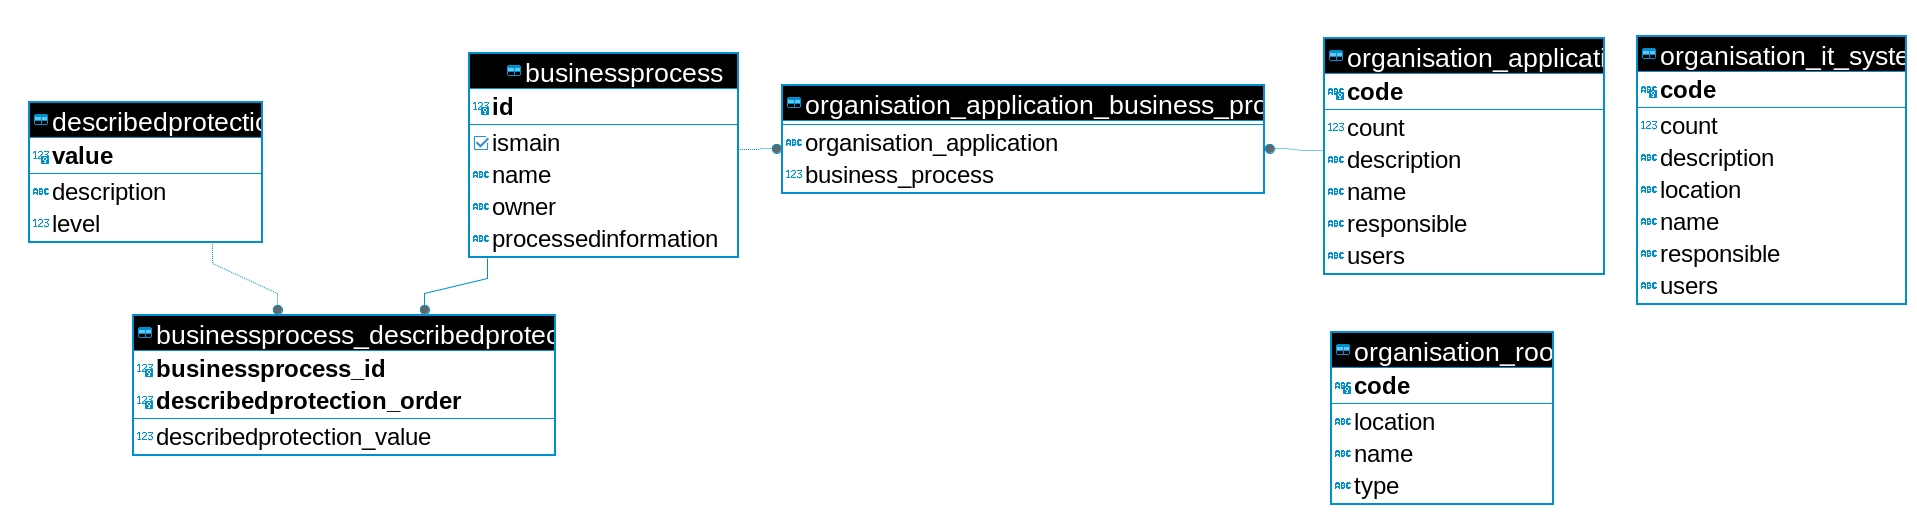
\includegraphics[width=11cm]{images/database-diagram-other-tables}
\end{frame}

\section{Záver}
\begin{frame}
  \frametitle{Zhrnuté: Čo sa nám podarilo?}
  \begin{itemize}
    \item analýza právnych požiadavkov
    \item \textit{proof-of-concept} systém
    \item vysvetlili sme manažérovi KIB jeho povinnosti
    \item uviedli a vysvetlili sme problematiky KIB manažérovi KIB
    \item získali sme od manažéra KIB informácie potrebné na vypracovanie bezpečnostnej dokumentácie KIB
  \end{itemize}
\end{frame}

\begin{frame}
    \frametitle{Ďalšia práca}
  \begin{itemize}
    \item systém nie je kompletný, je čiastočne implementovaný
    \item venovali sme sa zatiaľ iba zavádzaniu ISMS
    \item väčšia funkcionalita a pomoc manažérovi
    \item podrobnejšie v bakalárskej práci
  \end{itemize}
\end{frame}

\begin{frame}
  \frametitle{zdroje}
  \printbibliography[heading=none]
\end{frame}

\begin{frame}
  \frametitle{Koniec}
  Ďakujem za vašu pozornosť.
\end{frame}

\begin{frame}
  \frametitle{Posudky}
  \begin{itemize}
    \item \dots
  \end{itemize}
\end{frame}

\begin{frame}
  \begin{center}
    \Huge priestor na otázky
  \end{center}
\end{frame}


\end{document}
